\documentclass[12pt,upcase]{umlthesis}
\usepackage{lipsum}
\usepackage{natbib}
\usepackage{graphicx}
\usepackage{float}
\usepackage{hyperref}
\usepackage{amsmath}

% use fancyhdr, to enable page style stuff (below)
\usepackage{fancyhdr}
\setlength{\headheight}{15.2pt}
\renewcommand{\headrulewidth}{0pt}

\pagestyle{plain}

\begin{document}
\title{Two-Fluid Collisional Magnetohydrodynamic Modeling}
\author{Qusai Al Shidi}
\prevdegrees{B.S., University of Toledo (2008)}
\department{Department of Physics and Applied Physics}
\degree{Doctor of Philosophy}
\degreemonth{May}
\degreeyear{2019}
\thesisdate{May 1, 2019}
\supervisor{Ofer Cohen}{Assistant Professor}
\maketitle

%%%%%%%%%%%%%%%%%%%%%%%%%%%%%%%%%%%%%%%%
\begin{abstract}
	Since the discovery of space plasmas, the space science community have been deriving fluid models of plasmas to best suit their scenarios. The simplest case is the ideal magnetohydrodynamic (MHD) model which assumes a collisionless perfectly-conducting plasma. Multi-fluid collisional MHD gives each fluid its own set of MHD equations while using collisions to set frictional and resistive terms between them. An important case of this nature is the solar chromosphere. The high density and relatively cold plasma ensures collision times are shorter than magnetic time scales. Multi-fluid collisional MHD has many cases from the Earth's ionosphere to stellar atmosphere and having a good grasp of the physics is important in studying these plasmas.
\end{abstract}

%%%%%%%%%%%%%%%%%%%%%%%%%%%%%%%%%%%%%%%%
\begin{acknowledgments}
An acknowledgments page is optional.
\end{acknowledgments}


%%%%%%%%%%%%%%%%%%%%%%%%%%%%%%%%%%%%%%%%
\tableofcontents
\listoffigures
\listoftables

\chapter{Introduction}

The word `plasma' was first used by \citet{Langmuir1928} to describe oscillations in a gaseous electron medium~\citep{Tonks1967}. It is a state of matter that is can be described as an ionized gas. It is the most common form of baryonic matter in the universe. We default to plasma descriptions of the medium between stars and planets. The sun is, for example, made mostly of ionized hot plasma. It is made of plasma and shoots out supersonic plasma called the solar wind. This plasma does not entirely contact the Earth due to shielding resulting from the Earth's magnetic field. Due to plasma's ionization, it has a tendency to travel on magnetic field lines. This does not mean the Earth is completely shielded from the solar wind. Many space weather events are due to solar plasma's effect on the Earth and its magnetic field. The sun is a very active star that has spontaneous flares, coronal mass ejections (CME) and active regions. Thus spontaneous storms occur on Earth and our understanding of the sun and space plasmas is essential to protect ourself against storms.

In this dissertation, an attempt will be made to show the benefits and utility of multi-fluid magnetohydrodynamic (MHD) models. We will show that the solar chromosphere is a good case for this. The implementation will also be studied with careful use of good, modern computer science practices.

\section{The Sun}
\begin{figure}[h!]\label{fig:sunstructure}
	\centering
	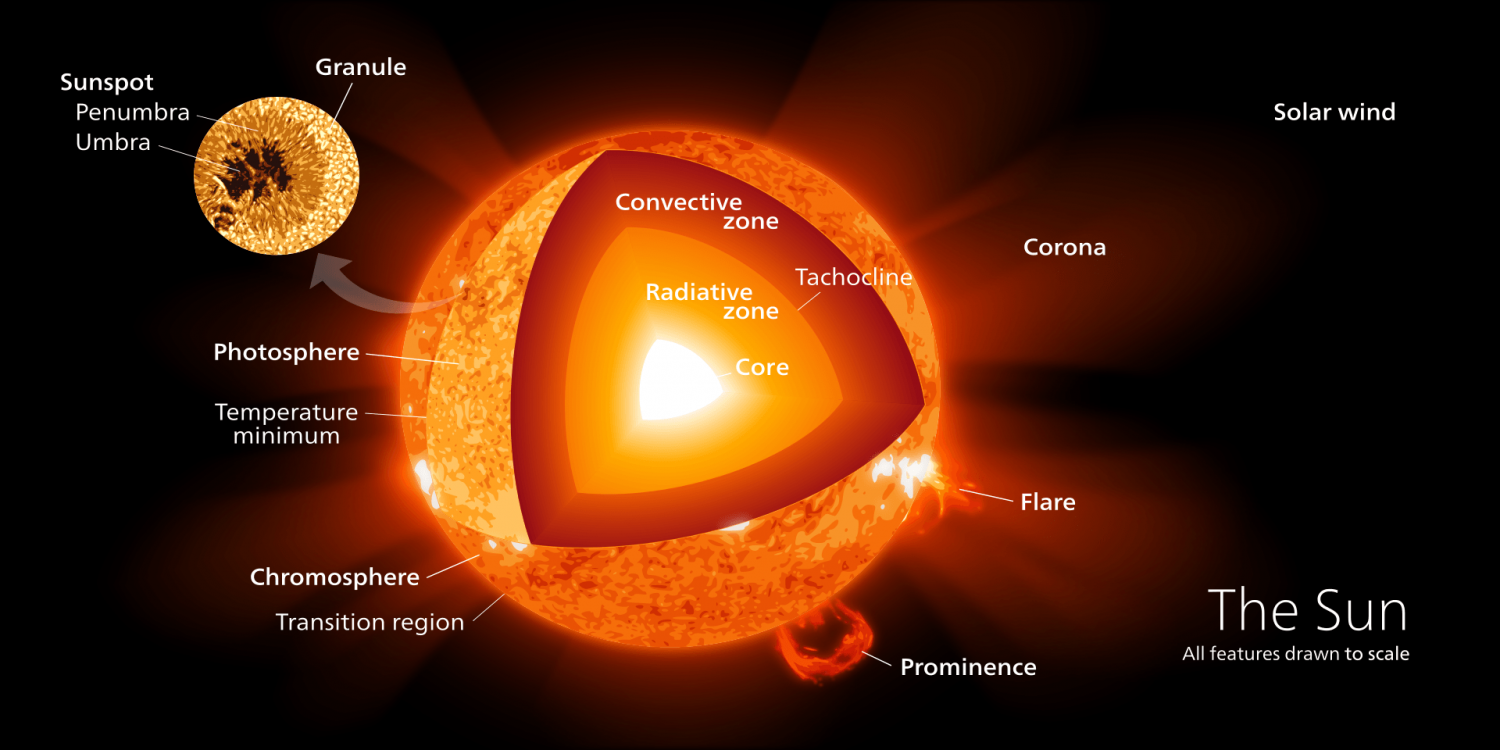
\includegraphics[width=1.0\linewidth]{sunstructure.png}
	\caption{A more complicated view of the sun's structure and layers. [{Image from \url{https://phys.org/news/2015-12-sun-energy.html}}]} % chktex 8
\end{figure}
Whenever we say `the sun' we do not mean any star---we mean \textit{our} star. The sun is a 4.6 billion year old yellow dwarf. It generates a lot of the energy we use for life on Earth. It creates this energy through nuclear fusion in its core, turning hydrogen into helium. The sun is mostly hydrogen with a small amount of helium and even smaller amounts of metal ions which require tremendous energy to fuse. The sun has six regions (from innermost to outermost): the core, the radiative zone, the covection zone, the photosphere, the chromosphere and the corona. The core is where the fusion happens. Here is where hydrogen is made into helium and other metals. The radiative zone and convection zone is where the energy travels radially upwards to wards the surface, the photosphere. The photosphere is the surface of the Sun. Here photons are trapped but the ones that do escape mimic black-body radiation (not perfectly). It is optically thick and is the white light we see when looking at the Sun. Above the photosphere is the atmospheric layer, the chromosphere, which we will go in much detail about in this dissertation. Above that, is the corona which is what gives the sun its tendrils and the hair we give our cartoon drawings of the sun.

\subsection{The Chromosphere}

The chromosphere is the interface between the surface, the photosphere, and the outer atmosphere, the corona. The plasma in it is partially ionized which means it consists of two kinds of plasma: ionized (charged) plasma, and neutral (uncharged) plasma. This means the charged plasma is affected by Lorentz forces while the uncharged plasma is not. This is a result of the temperature of the chromosphere and the composition of the plasma convected in the convection zone. The plasma has a high temperature in Earth standards but to the sun it is relatively cold. The temperature of the corona, which keep in mind is the outermost layer, is in the million of degrees in Kelvin. While most of the chromosphere and the photosphere is 5000K-6500K. This discrepancy in the temperature of the lower layers to the higher layers is called the coronal heating problem. The coronal heating problem is an outstanding problem in physics which makes understanding the chromosphere of special importance. Why is the corona hotter than the chromosphere?

\begin{figure}[ht!]\label{fig:chromoprofile}
	\centering
	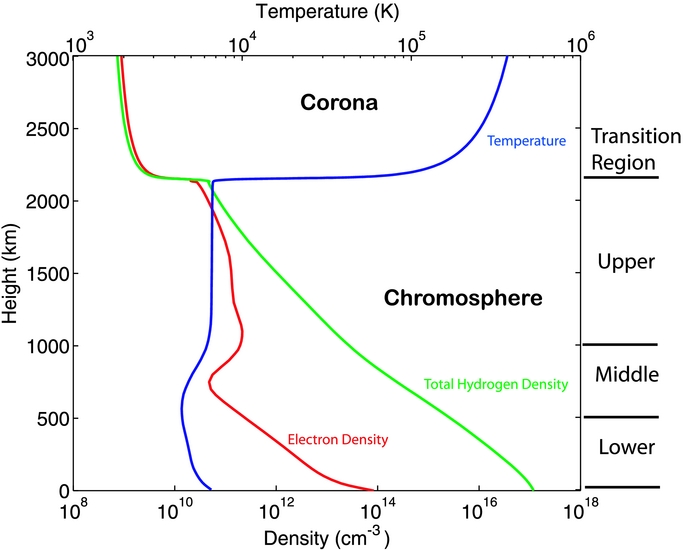
\includegraphics[width=0.75\linewidth]{chromoprofile.jpg}
	\caption{A view of the upper, middle and lower chromosphere. The chromosphere is partially ionized and is much colder than the corona (above the transition region).~\citep{Song2014,Avrett2008}}
\end{figure}


\section{Space Weather}

The term space weather refers to weather effects found above our immediate atmosphere which is conversely named terrestrial weather. It focuses on the conditions and changes found between the Sun, the Earth and even behind the Earth along its night time. The Earth's surface magnetic field strength is in the 0.5G range~\citep{Finlay2010} and that is strong enough to shield most of the solar wind headed our direction. However, magnetic reconnection events between the Earth's magnetosphere (the sphere of Earth's magnetic influence) and the interstellar medium allows solar wind particles to enter the Earth's atmosphere. This can manifest itself in harmless weather, like auroras, or more harmful weather, like geomagnetic storms.

\subsection{Motivation: A storm is coming}

In 1859, a famous (or infamous) geomagnetic storm hit the Earth. Fortunately, we did not sprawl global electrical power grids at the time or it would have had devastating effects. It was caused by a CME observed by Richard C. Carrington and was thusly named the Carrington Event. Depending on the strength of the geomagnetic storm (which happens frequently at higher/lower latitudes due to night side reconnection) it may reach mid-latitude areas which we habitate. Here geomagnetic storms due to the quick changes in magnetic fields and the law of induction cause ground induced currents (GIC) that can have damaging effects to any ground based electrical devices.

The Carrington event was our last encounter with a storm of that scale, that does not mean we have not had any near misses. In 2012, a coronal mass ejection that has the strength and size comparable to the previously mentioned Carrington event almost hit the Earth. It missed the Earth by nine days~\citep{Baker2013}. Unlike in 1859, the world of 2012 was filled with electrical power grids. The internet is part of our daily lives and still relies on ground based electrical wiring.



\subsection{Where does the chromosphere fit into this?}
%%%%%%%%%%%%%%%%%%%%%%%%%%%%%%%%%%%%%%%%

\chapter{Collisional Plasmas}

Although plasmas are classically defined as charged gasses, they can coexist with neutral plasma based on the temperature and pressure conditions surrounding them. This means we have two gas mediums, one with the ability to feel Lorentz forces and another that acts like a non-charged fluid. This will generate friction between the fluids when they are moving at different velocities. Due to collision rates being proportional to fluid density and temperature, there can exist a limit in which collision rates are larger than ionization/recombination rates of ions and therefore the fluid becomes collisional. In the reverse case a single-fluid is an apt description as the existence of two-fluids matters largely on the chemistry rather than the collisions. We will be focusing on hydrogen plasmas for our chromosphere case in Chapter~\ref{chap:chromosphere} and in that case two-fluids will be investigated.

\section{Magnetohydrodynamics}\label{sec:mhd}

Magnetohydrodynamics (MHD) is a fluid approximation of plasma popular amongst macroscopic studies of space plasmas. In order to arrive at the fluid approximation we must first look at the particles first and ensure the approximation is appropriate for our case. All of physics is a model and to go from the kinetic theory of plasmas by modelling particles to MHD plasmas by modelling fluids there must be a derivation since there are less assumptions in the kinetic theory than there are in MHD\@.

\subsection{Kinetic Theory}\label{sec:kinetictheory}

We start by assuming an ensemble phase space of particles $f(\textbf{x}, \textbf{v}, t)$ called the distribution function. $\textbf{x}$ is the location of the particle distribution in space, $\textbf{v}$ is the velocity distribution and $t$ is the time. To study the distribution function's evolution through time we take the full derivative with respect to time $\frac{df}{dt}$ which by the product rule turns out to be:

\begin{equation}
	\frac{\partial f}{\partial t} + \frac{\partial \textbf{x}}{\partial t} \cdot \nabla_{\textbf{x}} f + \frac{\partial \textbf{v}}{\partial t} \cdot \nabla_{\textbf{v}} f = {(\frac{\partial f}{\partial t})}_{collisions}
\end{equation}

This is called the Boltzmann equation. The term on the right hand side exists due to collisions changed the distribution function in its own way, this also include collisional ionization and other collisional effects that would change the distribution of particles. Simplifying the equation further by substituting how we expect the bulk particles to interact with fields we can get:

\begin{equation}
	\frac{\partial f}{\partial t} + \textbf{v} \cdot \nabla_{\textbf{x}} f + \frac{q}{m} (\textbf{E} + \textbf{v} \times \textbf{B}) \cdot \nabla_{\textbf{v}} f = {(\frac{\partial f}{\partial t})}_{collisions}
\end{equation}

Where $q$ is the charge of the particle, $m$ is the mass of the particle, $\textbf{E}$ is the electric field and $\textbf{B}$ is the magnetic field.

This is the kinetic theory of plasmas. The assumptions made here are probability distributions of particles instead of singular particle effects. There are simulations and codes that model particles directly but because of the large memory size of such simulations the region of study must be very small. 

\subsection{Moments of the Distribution}\label{sec:moments}

In order to arrive at the macroscopic variables we must make an assumption about the distribution of the fluid. This is the most fundamental assumption of MHD is that the distribution of the particles are behaving like a Maxwellian velocity distribution. If it is not the case that the velocity distribution is Maxwellian then the approach of MHD is challenged and must be rewritten and integrated differently. The Maxwellian velocity distribution is common in space plasmas that are in thermal equilibrium with itself which lends to the popularity of MHD\@.

\begin{equation}
	f(v) = n {(\frac{m}{2\pi k_B T})}^{3/2} \exp{(-\frac{mv^2}{2k_B T})}
\end{equation}

Where $v = |\textbf{v}|$ is the speed, $k_B$ is the Boltzmann constant and $T$ is temperature. This is assuming a Maxwellian velocity distribution over a thermal equilibrium and a thermal speed.

To arrive at the MHD equations we start to take the `velocity moments' of the equations in order to have macroscopic variables that don't depend on phase speed.

\begin{equation}
	{Moment}_a(\textbf{x}, t) = \int{\textbf{v}^a f(\textbf{x}, \textbf{v}, t)}d\textbf{v}
\end{equation}

Here $a$ is the order of the moment. The first few moments are of interest. The zeroth moment is the continuity equation.

\begin{equation}\label{eq:continuityequation}
	\frac{\partial n_s}{\partial t} + \nabla \cdot (n_s \textbf{v}_s) = {(\frac{\delta n_s}{\delta t})}_{source}
\end{equation}

Each species, $s$, of fluid has its own continuity equations but may be related by the source terms. The source terms come from integrating the collisional ionization, radiative recombination, etc.

The first order moment will give us the momentum equations:

\begin{equation}\label{eq:momentumequation}
	\frac{\partial n_s \textbf{v}_s}{\partial t} + \nabla \cdot (n_s \textbf{v}_s \textbf{v}_s + \textbf{P}_s ) -n_s \frac{q}{m_s}(\textbf{E} + \textbf{v}_s \times \textbf{B}) = {(\frac{\delta n_s \textbf{v}_s}{\delta t})}_{source}
\end{equation}

Where $\textbf{P}_s$ is the kinetic pressure tensor and can be simplified to the ideal gas law $P_s\textbf{I} = n_s k_B T_s \textbf{I}$ if applicable. The source terms due to the zeroth order also exists here as well as frictional terms that may appear in multifluid cases. It is apparent that this equation is fluid-like, a form of the Navier-Stokes equation and hence the naming of these equations as hydrodynamic.

To close the system equations we need one more for the pressure shown previously. So integrating for the second moment gives:

\begin{equation}\label{eq:energyequation}
	\frac{\partial E_s}{\partial t} + \nabla \cdot (\textbf{v}_s E_s) + \nabla \cdot \textbf{q}_s = {(\frac{\delta E_s}{\delta t})}_{source}
\end{equation}

Where $q$ is the heat flow tensor which can be approached in multiple ways and $E$ is the total energy:

\begin{equation}\label{eq:energy}
	E_s = e_s + \frac{1}{2} m_s {v^2}_s + E_{potential}
\end{equation}

Here $e$ is the internal energy and the potential energy is based on the momentum equation's extra acceleration terms like the fields or gravitational potential energy if included.

\subsection{Multi-fluid MHD}\label{sec:multifluidmhd}

In order to make our code capable to solve the equations shown in the previous section (Section~\ref{sec:moments}) further approximations must be done. The three fluids of interest in a hydrogen plasma that includes neutrals are hydrogen ions, electrons and neutral hydrogen. Our plasma is collisional and in partially ionized plasmas we can use the Krook collision term.

\begin{equation}\label{eq:krook}
	{(\frac{\delta f}{\delta t})}_{collisions} = \nu_n (f_n - f)
\end{equation}

Where subscript $n$ is the neutral species and $\nu$ is the collision rate. We can find the collision rate simply by using the collision cross-section of neutral particles and the average thermal speed. The average thermal speed is used because temperature in the case of MHD is based on the `peculiar' speeds of the particles (i.e.\ particles with velocity other than that of the bulk plasma). This way peculiar velocities contribute to collisions because if both fluids are moving in the same direction.

\begin{equation}\label{eq:collisionrate}
	\nu_n = n_n \sigma_n <v>
\end{equation}

The thermal speed is a function of temperature and under the Maxwellian velocity distribution assumption, $sigma$ is the collisional cross-section which can be found in the literature through experiments. The collisional cross-section between ion and electrons include Coloumb effects as well.

The moment equations (Equation~\ref{eq:continuityequation}-\ref{eq:energyequation}) for the three species will look like this:

\begin{equation}\label{eq:icontinuity}
	\frac{\partial n_i}{\partial t} + \nabla \cdot (n_i \textbf{v}_s) = S - L
\end{equation}

\begin{equation}\label{eq:econtinuity}
	\frac{\partial n_e}{\partial t} + \nabla \cdot (n_e \textbf{v}_s) = S - L
\end{equation}

\begin{equation}\label{eq:econtinuity}
	\frac{\partial n_n}{\partial t} + \nabla \cdot (n_n \textbf{v}_s) = L - S
\end{equation}

\begin{equation}\label{eq:imomentum}
	\frac{\partial n_i \textbf{v}_i}{\partial t} + \nabla \cdot (n_i \textbf{v}_i \textbf{v}_i + \textbf{P}_i ) - n_i \frac{q_i}{m_i}(\textbf{E} + \textbf{v}_i \times \textbf{B}) = - \sum_{i \neq s} [n_i \nu_{is}(\textbf{v}_i - \textbf{v}_s)] + \frac{1}{m_i} (S m_n \textbf{v}_n- L m_i \textbf{v}_i)
\end{equation}

\begin{equation}\label{eq:emomentum}
	\frac{\partial n_e \textbf{v}_e}{\partial t} + \nabla \cdot (n_e \textbf{v}_e \textbf{v}_e + \textbf{P}_e ) - n_e \frac{q_e}{m_e}(\textbf{E} + \textbf{v}_e \times \textbf{B}) = - \sum_{e \neq s} [n_e \nu_{es}(\textbf{v}_e - \textbf{v}_s)] + \frac{1}{m_e} (S m_n \textbf{v}_n - L m_e \textbf{v}_e)
\end{equation}

\begin{equation}\label{eq:nmomentum}
	\frac{\partial n_n \textbf{v}_n}{\partial t} + \nabla \cdot (n_n \textbf{v}_n \textbf{v}_n + \textbf{P}_n ) = - \sum_{n \neq s} [n_n \nu_{es}(\textbf{v}_n - \textbf{v}_n)] + \frac{1}{m_n} (L(m_i\textbf{v}_i+m_e\textbf{v}_e) -S m_n \textbf{v}_n)
\end{equation}

\chapter{Implementation}\label{chap:implementation}

Computational fluid dynamics is a well studied field in computer science, numerics and engineering. Many of its principles can be appled to MHD due to the fluid nature of its equations. We will be focusing on only the ones implementedd in the code my for this dissertation, the Collisional Multi-Fluid ion (CoMFi) code made for the chromosphere case which will be explored in more detail in the upcoming chapter (Chapter~\ref{chap:chromosphere}). The code is an ever-evolving code that uses Graphical Processing Units (GPUs) instead of the common CPUs you see for MHD codes. This is to implement MHD that makes use of the frontiers of computer technology. GPUs were made for graphical operations in video games. This means they are specifically designed to be very fast at matrix rotations, translations and other linear algebra. In this chapter we will explore proper general purpose GPU programming techniques for solving differential equations and the schemes used alongside it. CoMFi is written in C++ using ViennaCL for GPU linear algebra template programming and Armadillo for setting up the matrices on the CPU (the reason for this will be discussed in).

\section{Schemes}

CoMFi uses the conservative MHD equations therefore conservative schemes are of interest. This makes use of the conservative variables unknowns as opposed to the primitive variables ($n v$ as opposed to $v$). This way we can use a finite-volume-method and conserve these quantities to the machine rounding error. Conservative schemes are also known to do well at capturing shocks and the chromosphere is a region where we expect such shocks to exist.

\begin{equation}\label{eq:geneuler}
	\frac{\partial \textbf{u}}{\partial t} + \nabla \cdot \textbf{F(u)} = 0
\end{equation}

The above equation is a general euler equation demonstrating a conservation law problem. The quantity to be conserved is $\textbf{u}$ and is a function the flux $\textbf{F}$. We will be considering the linear case for simplicity however MHD has demonstrably non-linear terms as the flux (e.g. Equation~\ref{eq:imomentum}) but it can easily follow from this linear case. The point is to show the total volume is conserved:

\begin{equation}\label{eq:geneulerint}
	\frac{d\textbf{u}}{dt} + \frac{1}{V} \oint \textbf{F} \cdot \textbf{n} dS
\end{equation}

In codes designed to solve differential equations numerically we must decide on the discretization. Since we are using a finite-volume-method we are discretizing the domain by cells with density quantities in them. The code is discretized in cells existing in cartesian coordinates (rectangular cells) so we are tasked to find the values of the variables at the cell faces in order to conserve the volume.

We would also like a total-variation-diminishing (TVD) scheme, this is because spatial derivatives are approximated on a computer. If we take a taylor series of a derivative from one cell to another and compare with an approximate derivative like $\frac{u(x+\Delta x)-u(x-\Delta x)}{2\Delta x}$ we see that there are many higher order terms missing. Taking the fourier analysis of these terms show that any high-frequency errors may compound (sometimes referred to as spurious oscillations). This can be fixed by schemes that ensure the total variation $TV$ is diminishing.

\begin{equation}\label{eq:tvd}
	\frac{dTV}{dt} = \frac{d}{dt} \int \lvert \frac{\partial u}{\partial x} dx \leq 1
\end{equation}

Therefore, for the the purpose of our code, we will use the Total-Variation-Diminishing Monotonic Upwind Scheme for Conservation Laws (TVD-MUSCL).

\subsection{Flux limiters}

To conserve the cell's quantities we must be able to approximate the quantities on the cell edges. At the same time we must perserve monotonicity to avoid the oscillations. This can be achieved through flux limiters. The utility of the flux limiters is to turn the scheme into a first-order upwind scheme in sharp discontinuities and a high-resolution scheme when the solution is smooth.

\begin{equation}\label{eq:fluxlimiter}
	u_{j+1/2} = u_j + \frac{1}{2} \phi(r_j) (u_{j+1} - u_j)
\end{equation}
\begin{equation}
	r_j = \frac{u_j - u_{j-1}}{u_{j+1} - u_j}
\end{equation}

Subscript $j$ is the discretized cell location with quantity $u$. The ratio of successive gradients $r$ determines how strongly the flux limiter acts to find the extrapolated cell edge variable. The flux limiter $\phi$ includes the cells around edge more readily the smoother the solution is ($r>0$), or sharp it is ($r<0$) in which case the flux limiter is zero ($\phi=0$). These are the properties flux limiters must abide in order to turn the scheme upwind in sharp gradients or high-resolution in smoother gradients. The above equation is a linear reconstruction of a cell edge. Other reconstructions exist but are more diffusive and avoids the shock-capturing goal of the code.

We have some freedom in choosing how to set the flux limiter. Many flux limiters have been made and studied in the past. The simplest flux-limiter is the minmod.

\begin{equation}\label{eq:minmod}
	\phi_{minmod}(r) = \max(0, \min(1, r)), \lim_{r \to \infty} \phi(r) = 1
\end{equation}

The CoMFi code provides several flux limiters and finding the best one is a matter of trial and error. The limiter used by default is the van Albada limiter.

\begin{equation}\label{eq:vanalbada}
	\phi_{va}(r) = \frac{r^2 + r}{r^2 + 1}, \lim_{r \to \infty} \phi(r) = 1
\end{equation}

Implementing these on a computer however is not a trivial task. Many initial conditions require the entirety of the domain be the same number for instance. In that case we get an $r = \frac{0}{0}$ and this causes a computer to return NaN (not a number). Setting to $r=0$ is approriate but requires extra coding. A work around is to add a small number $\epsilon$ to the denominator known as the machine epsilon to avoid these cases.

\begin{equation}
	r_j = \frac{u_j - u_{j-1}}{u_{j+1} - u_j + \epsilon(u_{j+1} - u_j + 1)}
\end{equation}

\subsection{TVD-MUSCL}

The TVD-MUSCL scheme reconstructs `left' ($L$) and `right' ($R$) states of the cell edge variables. 

\begin{equation}
	u^L_{j-1/2} = u_{j-1} + \frac{1}{2} \phi(r_{j-1}) (u_j - u_{j-1})
\end{equation}
\begin{equation}
	u^L_{j+1/2} = u_{j} + \frac{1}{2} \phi(r_{j}) (u_j - u_{j-1})
\end{equation}
\begin{equation}
	u^R_{j-1/2} = u_{j} + \frac{1}{2} \phi(r_{j}) (u_{j+1} - u_{j})
\end{equation}
\begin{equation}
	u^R_{j+1/2} = u_{j+1} + \frac{1}{2} \phi(r_{j+1}) (u_{j+1} - u_{j})
\end{equation}

With the left and right extrapolated variables we may construct a flux.

\begin{equation}
	F^*_{j-1/2} = \frac{1}{2} ([F(u^R_{j-1/2})+F(u^L_{j-1/2})] - \lambda_{j-1/2}[u^R_{j-1/2}-u^L_{j-1/2}])
\end{equation}
\begin{equation}
	F^*_{j+1/2} = \frac{1}{2} ([F(u^r_{j+1/2})+F(u^l_{j+1/2})] - \lambda_{j+1/2}[u^r_{j+1/2}-u^l_{j+1/2}])
\end{equation}

Here $F u = \lambda u$ are the eigenvalues of the variables. This in physical terms means the largest wave speeds of the system. Typically for the ion plasma it is the fast-mode speed and for the neutrals it is the sound speed. It's important to note in conservative MHD this is only the wave speed ($c_{fast}$) and not the same as the fastest speed of information propagation ($v+c_{fast}$). The diffusive terms proportional to $\lambda$ are meant to avoid the oscillations and if they are larger than they need to be the solution will be more diffusive.

\section{Time Integration}

\section{Structure}

\subsection{Data Structure}

When using the semi-implicit method a linear system $Ab^{n+1}=b$ must be solved. We must think of an approriate ordering of our vector in terms of the where the unknowns must be in the elements of the vector. For GPU programming in order to take advantage of its matrix operations speeds due to its many cores we must also be easily able to change back and forth between matrix and vector form between the implicit and explicit portions of the solution. A good ordering for a two-dimensional domain looks like this:

\begin{equation}
	b =
\begin{bmatrix}
	u_{0,00} \\
	\vdots \\
	u_{0,i0} \\
	\vdots \\
	u_{0,ij} \\
	\vdots \\
	u_{w,ij} \\
\end{bmatrix}
\end{equation}

The subscripts $i$ and $j$ describe the location of the cell in the $x$ and $y$ axis respectively and $w$ are the scalar unknowns.

\begin{equation}
	u_w = 
	\begin{bmatrix}
		B_x \\
		B_{\perp} \\
		B_z \\
		n_i \\
		n_n \\
		n_i V_x \\
		n_i V_{\perp} \\
		n_i V_z \\
		n_n U_x \\
		n_n U_{\perp} \\
		n_n U_z \\
		T_i \\
		T_n \\
		\Phi
	\end{bmatrix}
\end{equation}

This can be easily resized into a matrix of the form:

\begin{equation}
	B =
	\begin{bmatrix}
		u_{0,00} & \cdots  & u_{w,00} \\
		\vdots   & \ddots & \vdots \\
		u_{0,i0} & \cdots & u_{w,i0} \\
		\vdots   & \ddots & \vdots \\
		u_{0,ij} & \cdots  & u_{w,ij}
	\end{bmatrix}
\end{equation}

This has the benefits of making good use of GPU programming by using the parallelism found in matrix operations. This also means you can share boundary conditions by taking or providing rows for this matrix in chunks. You can do operations on specific unknowns by taking the approriate column.

\subsection{Normalization}

\chapter{Case: Chromosphere}\label{chap:chromosphere} 

\chapter{Conclusion}\label{chap:conclusion}
%%%%%%%%%%%%%%%%%%%%%%%%%%%%%%%%%%%%%%%%
%\nocite{*}
\bibliographystyle{plainnat}
\bibliography{phd-thesis}

%%%%%%%%%%%%%%%%%%%%%%%%%%%%%%%%%%%%%%%%
\appendix
\chapter{Appendix Chapter}
\lipsum[2]

\end{document}
